\documentclass{standalone}
\usepackage{tikz}
\usepackage{pgfplots}
\usetikzlibrary{patterns, calc}

\begin{document}
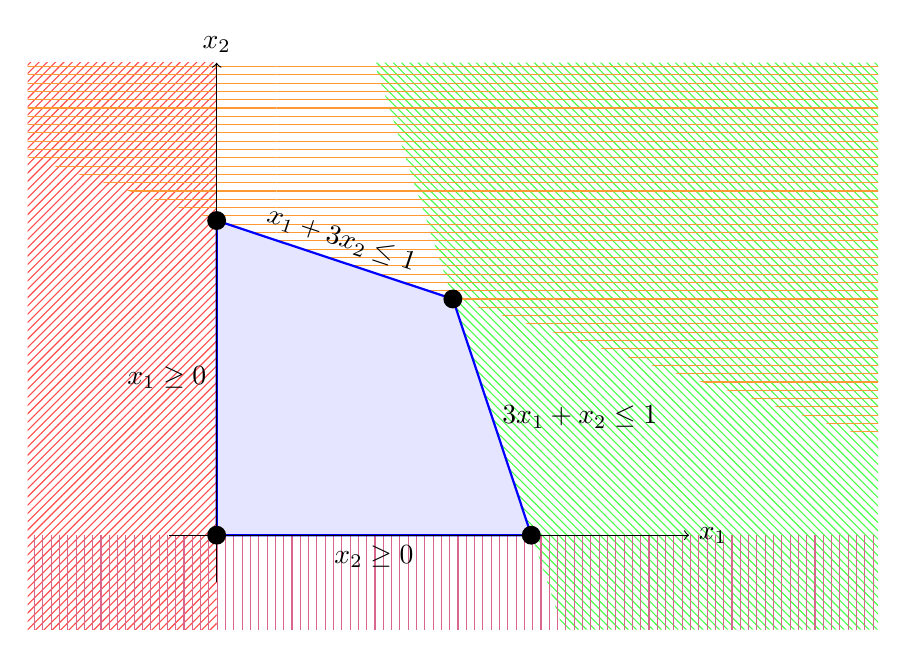
\begin{tikzpicture}[scale=12]

  % Define points of polyope
  \coordinate (A) at (0, 0);
  \coordinate (B) at (0.333, 0);
  \coordinate (C) at (0.25, 0.25);
  \coordinate (D) at (0, 0.333);

  % 1. shade left side 
  \fill[pattern=north east lines, pattern color=red!70]
    (-0.2, -0.1) rectangle (0, 0.5);

  % 2.  shade right side 
  \fill[pattern=north west lines, pattern color=green!70]
    (0.3667, -0.1) -- 
    (.1667, 0.5) --
    (.7, .5) --
    (.7, -.1) -- cycle;

  % 3. shade above
  \fill[pattern=horizontal lines, pattern color=orange!80]
    (-.2, .4) --
    (-.2, .5) --
    (0.7, 0.5) --
    (0.7, .1) -- cycle;

  % 4. x_2 >= 0 → shade below (x_2 < 0)
  \fill[pattern=vertical lines, pattern color=purple!60]
    (-0.2, -0.1) rectangle (0.7, 0);

  % Draw polxytope
  \filldraw[fill=blue!10, draw=blue, thick]
    (A) -- node [below] {$x_2 \geq 0$} 
    (B) -- node [right] {$3x_1 + x_2 \leq 1$}
    (C) -- node [sloped, above] {$x_1 + 3x_2 \leq 1$}
    (D) -- node [left] {$x_1 \geq 0$} cycle;

  % Points
  \foreach \point/\name in {(A)/A, (B)/B, (C)/C, (D)/D}
    \fill \point circle[radius=0.01];

  % Ax_1es
  \draw[->] (-0.05, 0) -- (0.5, 0) node[right] {$x_1$};
  \draw[->] (0, -0.05) -- (0, 0.5) node[above] {$x_2$};


\end{tikzpicture}
\end{document}
